%!TEX root = ../main.tex

% Name of the model: Transfer Learning For Time Series Imputation
\section{Overview}
In this chapter the proposed work of \textbf{Transfer Learning For Time Series Imputation} is described with the system models, analytical models, flow diagrams, model architecture, trained model symmary along with the discussion about every components in detail.

\section{System Model}

System model is such that once we achive the desired level of model accuracy and loss value that model are deployed in the real environment so that it get used and also trained in online environment which is that it self correct and make the system self sufficient .Our system model consists of the following components.

\subsection{Sensing Layer}
Sensors and actuators in this layer collect data from the environment in this layer.
Also, it provides the interface to the real world to interact with the environment and provide impact in the physical world. It helps in both collecting data from the environment and to provide action that results in the making system work properly with in the sync.

\subsection{Network Layer}
Data collected by the sensing layer is transported to the computing devices and processing and control system using Network Layer. This layer is used for transporting the processed and to be processed data to and fro from on end to the other end. Many protocols and networks like MQTT COAP can be used easily.

\subsection{Data Processing Layer}
The data processing layer is the layer of IoT Architecture where all the computing of the system occurs. Our paper tries to solve the problem all of which lies here. It is the part of processing unit as shown in Figure. \ref{fig:system-model}

\underline{Nature of IoT data} - IoT systems generates high-volume, streaming, location, and time-specific this type of data is called time-series data. 
We would be deploying our fault-tolerance system in this layer only.

\subsubsection{Fault tolerance layer}
In this layer, we predict the missing values that our sensors don’t able to collect. This may be due to many various reasons like sensor failure, network disturbance, battery discharge etc. this is the part where the action according to the predictions is taken. It may be some alarm initiation some improvement logic or simply update the record in the database. This is also the part of the processing unit as shown in Figure. \ref{fig:system-model}

\subsection{Application layer}
The application layer is the layer where the user interacts with the system or the machine interface takes action based on the output of the IoT system. 

Application layer can be made in any framework that working and nature of problem. In the current simulation scenario as the pollution data is taken for the reference it is more feasble to make a web interface where an user can see the real time monioring of the various weather and pollution parameters and if required can take action based on the results shown in the dashboard. For making the dashboard any front end framework can be used like Angular or React where it is very easy to build user interfaces with single page application. For the backend python framework like django or flask can be used as it will help in predicting and implementing the machine learning models on the cloud environment.
\\
Server side application programmable interface and front end dashboard can be connected with the any real time network interface. The one which would work feasible is socket. Other protocols like MQTT or COAP can also be used.

In the fault tolerance layer, we have generated a machine learning model in that we can generate inferences from and also train the model in real-time.




\begin{figure}[ht]
	\centering
	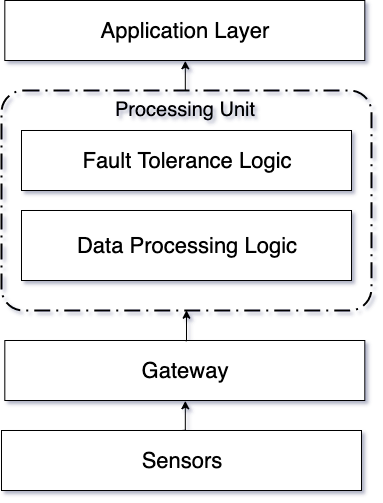
\includegraphics[width=0.5\textwidth]{images/system-model.png}
	\caption{System Model}
	\label{fig:system-model}
\end{figure}

\section{System Flow}
In this section the flow of the data and precessing and imputation processes are described. The figure \ref{fig:system-flow-diagram} dipicts the system flow diagram in the form of data flow diagram.

\begin{figure}[ht]
	\centering
	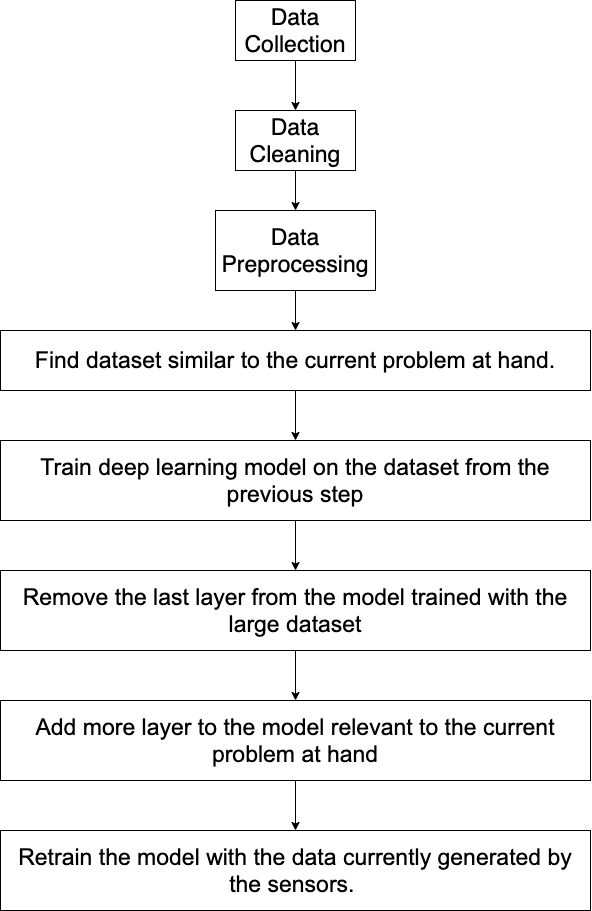
\includegraphics[width=0.8\textwidth]{images/system-flow-diagram.png}
	\caption{System Flow Diagram of Transfer Learning For Time Series Imputation}
	\label{fig:system-flow-diagram}
\end{figure}




\subsection{Data Collection}

For this demonstration and testing the approach proposed 
PM2.5 Data of two chinese are taken. This data is taken from UCI machine learning repository. It is very famous source for dataset for academic purposes. It contains many famous machine learning dataset widely used for academic and research perposes. Some of them are IRIS Flower Dataset, Titanic Survival dataset, etc. The two cities PM2.5 values data are taken from a dataset containing PM2.5 values of five chinese cities named "PM2.5 Data of Five Chinese Cities Data Set". Description of the dataset used is given below.

\underline{Dataset abstract} This hourly data set contains the PM2.5 data in Beijing, Shanghai, Guangzhou, Chengdu and Shenyang. Meanwhile, meteorological data for each city are also included.

The table \ref{tab:dataset-characteristic} describe the nature of the dataset.

\begin{table}[ht]
\centering
\begin{tabular}[widht=\textwidth]{|l|l|}
\hline
Data Set Characteristics &  Multivariate, Time-Series \\
Number of Instances & 52854 \\
Area & Physical \\
Attribute Characteristics & Integer, Real \\
Number of Attributes & 86 \\
Date Donated & 2017-07-18 \\
Associated Tasks & Regression \\
Missing Values? & Yes \\
Number of Web Hits & 81692 \\
\hline

\end{tabular}
\caption{Dataset Characteristics}
\label{tab:dataset-characteristic}
\end{table}

The table \ref{tab:dataset-attributes} describe attributes and features of the attributes of the dataset.


% Feature Table
\begin{table}[ht]
\centering
\begin{tabular}[widht=\textwidth]{|l|l|}
\hline

No & row number \\
year & year of data in this row \\
month & month of data in this row \\
day & day of data in this row \\
hour & hour of data in this row \\
season & season of data in this row \\
PM & PM2.5 concentration  \\
DEWP & Dew Point (Celsius Degree) \\
TEMP & Temperature (Celsius Degree) \\
HUMI & Humidity (\%) \\
PRES & Pressure (hPa) \\
cbwd & Combined wind direction \\
Iws & Cumulated wind speed (m/s) \\
precipitation & hourly precipitation (mm) \\
Iprec & Cumulated precipitation (mm) \\
\hline
\end{tabular}
\caption{Dataset Attributes}
\label{tab:dataset-attributes}
\end{table}

The two cities selected out of 5 are Beijing and Shanghai. Beijing data is used as the data set with large values and the Shanghai data is considered as the realtime data for which deep learning model need to be developed. This data is traind both without using transfer learning and with the transfer learning applied.

\subsection{Data Cleaning}

Data cleaning is a process of sanitising the data available with us so that its usabilituy may increase. There is a very famous phrase in data science garbage in garbage out. So data cleaning is very important step in any data related work.

Dataset contains many missing values which currently cannot make use of as it is so the missing values columns are dropped from the dataset managing the consistency in the dataset and the cleaned datase is used for the further processing.

Following method of the pandas is used for the cleaning the data.

\begin{verbatim}
pm25_beijing = df1.iloc[:, 5].dropna().values[:].reshape(-1, 1)

pm25_shanghai = df2.iloc[:, 9].dropna().values[:600].reshape(-1, 1)
\end{verbatim}

\subsection{Data Preprocessing}

\subsubsection{Loading the data}
The dataset is stored on a github repository so that it can be easily accessed through a link anywhere the code is running. The only need would be internet access while runing the code.

Matplotlib library is used for loading the data in the python environment. 

\begin{verbatim}
import matplotlib.pyplot as plt
URL_beijing = "LINK_OF_GITHUB_CSV_FILE"
df_beijing = pd.read_csv(URL_beijing)
\end{verbatim}

\subsubsection{Removing unnecessary data}
Actually the dataset consisted of various featue about the weather but for simplicity all other attributes except PM2.5 were removed.

\subsubsection{Scaling the data}
The PM2.5 values are not in the range of -1 to 1 so these values are scaled down to -1 to 1 range so that the can be fed to the machine learning algorithm later.

Scikit learn StandardScaler function is used for scaling the data down.

\begin{verbatim}
from sklearn.preprocessing import StandardScaler
scaler_beijing = StandardScaler()
scaler_beijing.fit(pm25_beijing)
pm25_beijing = scaler_beijing.transform(pm25_beijing)
\end{verbatim}

\subsubsection{Making dataset as input output pair for training}

There are several ways of doing this the one best technique of doing this. One method is discussed earlier.
For this sliding window protocol is used for making this data as supervised learning dataset so that it can be trained.

\begin{verbatim}
N = 20
O = 5
P = 20

X_beijing = []
y_beijing = []

for i in range(len(pm25_beijing) - (N + O + P)):
    temp = []
    temp1 = pm25_beijing[i : i+N]
    temp2 = [0 for _ in range(O)]
    temp3 = pm25_beijing[i+N+O : i+N+O+P]
    X_beijing.append(np.append(np.append(temp1, temp2), temp3))
    y_beijing.append(pm25_beijing[i+N : i+N+O].reshape(O))
\end{verbatim}


Here N is the length of the left slide length, O is the output length, i.e., for how many timestamp we want to predict the output, and P is the length of the right slide length.

The X data is prepared as to consist of left slide length from the sequence of data available for the output lenth 0 is filled in the sequence and at last the right slide length data is attached.

The y of the dataset is prepared by taking the actual values of the timestamp values of the O length datapoints.


\subsection{Finding Similar Dataset}
As the transfer learning to work for the WSN or IOT data it is necessary to find some dataset similar to the problem at hand that need to be solved. This type of cases can be very simmilar to real world such that a new thermal plant is need to be installed in any area and there is need for some fault toulerence logic for that but not have enough data to train the deep learning model for that. For that similar dataset can be picked from any similar thermal plant sensors.

For training for the shanghai PM2.5 value prediction Beijing data is used as training point for applying the transfer learning.

\subsection{Training deep neural network}

\subsubsection{Spliting the dataset into training and test sets}
Before feeding the data to the model the first step is to split the data into training and the test set so that model performance can be measured.\\

Scikit-Learn library model selection model train test split function is used for spliting the dataset into the training and testing values.\\

Code for this splitting is provided below\\

\begin{verbatim}
from sklearn.model_selection import train_test_split
X_train, X_test, y_train, y_test = train_test_split(X_beijing, y_beijing)
\end{verbatim}
\subsubsection{Training}

The first step of applying transfer learning is to train the model with huge amount of data available from any source which give the huge amount of data. The dataset for transfer learning training is picked in the previous section, that is Beijing city data. The deep learning model is first trained on the Beijing PM2.5 values dataset that contains data from previous several years.

\subsection{Removing last layer of DNN}
For applying the transfer learning to with the existing model the first step is to remove the last layer of the trained model so that new model with its features and attributes can be coded. the main motive of removing the last layers of the DNN to apply transfer learning is to incorporate the feature of the dataset one we are trying to train now.

\subsection{Adding more layer to the DNN}
The next step of applying the trasfer learning is to add more layer to the model from the previous step so that the new feature can be incorporated and trained again for the new dataset. 

*Note: The last two steps can be ignored if nature and nature of data is ditto same.

\subsection{Retraining the model}
When new layer is added to the model now it can be trained on the data available now for new sensor on new location. Training can be in any manner, i.e., online training or batch training.

\section{Model Architecture}

The two models is selected for applying transfer learnig for this proposed work. Figure \ref{fig:model-summary} describes the model summary of the two models.

\subsection{SSIM (Sequence to Sequence Imputation Model)}

	LSTM is a special kind of RNN(Recurrent Neural Network) which exploit the pattern in the data which makes. It has a memory unit which remember the previous sequence in the memory.
	SSIM is an encoder decoder model which is generally used in natural language processing for machine translation and it can be used here for time series imputation. Figure \ref{fig:shanghai-ssim-model-summary} Describe this architecture of the SSIM model.

	The SSIM model architecture contains the followin layers.
	\subsubsection{Bidirectional LSTM layer}
	It is a bidirectional LSTM layer to exploit the data in both the direction in forward along with backwards. 

	There are 128 neurons used in the Bidirectional LSTM layer.

	\subsubsection{Attenttion Layer}
	This is a layer used in Encoder Decoder model to focus on certain specific part of the sequence which are more relevant to the application and provides better results.
	An analogy of this is found in the image processing where the task is to identify the object in the image. Since the object in the image can be found in certain part of the photograph it need to focus on that part of the photo to identify the object. Figure. \ref{fig:attention} describes this proces of attention mechanism in terms of computer vision.

	\begin{figure}[ht]
		\centering
		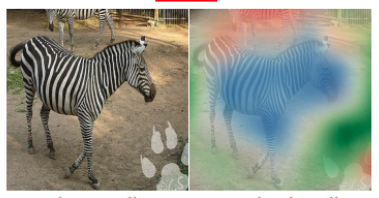
\includegraphics[width=0.8\textwidth]{images/attention.png}
		\caption{Attention Mechanism in terms of computer vision}
		\label{fig:attention}
	\end{figure}

	\subsubsection{LSTM Layer}
	This is a simple LSTM layer in the SSIM model comparising the decoder of the encoder decoder system. This layer is used for decoding the sequence generated by the input.

	\subsubsection{Dense Layer}
	This layer is used for maping the output sequence to the desired number of output timestamp values needed by the model.



\subsection{CNN (Convolutional Neural Network)}

	Convolution neural network is basically the applied in the field of image recognition and computer vision to find pattern in the image and label according to the labels given to it. Figure \ref{fig:shanghai-ssim-model-summary} describes the model summary of the CNN model.

	\subsubsection{Conv1D Layer}
		This is the first layer of the CNN model containing for learning the pattern in the data. It contains with 64 filters, kernal size is 3 and relu activation function is used.

	\subsubsection{MaxPooling Layer}
		Maxpooling layer is used to down sample input to eleminate the overfitting the training data.

	\subsubsection{Flatten Layer}
		The flatten layer is used to change the shape of the input to the 1D sequence of data.

	\subsubsection{Dense Layer X 2}
		Two Dense Layer is used one with 50 neurons and another with the 5 neurons to generate the output sequence of the desired length (5 timestamp)


\begin{figure}[ht]
	\centering
	\begin{subfigure}[b]{0.80\textwidth}
		\centering
		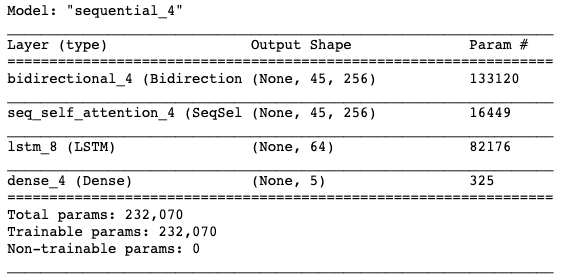
\includegraphics[width=\textwidth]{shanghai-ssim-model-summary}
		\caption{Shanghai SSIM Model Summary}
		\label{fig:shanghai-ssim-model-summary}
	\end{subfigure}
	\hfill
	\begin{subfigure}[b]{0.80\textwidth}
		\centering
		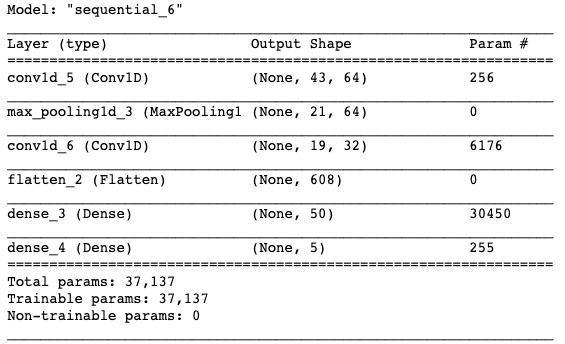
\includegraphics[width=\textwidth]{shanghai-cnn-model-summary}
		\caption{Shanghai CNN Model Summary}
		\label{fig:shanghai-cnn-model-summary}
	\end{subfigure}
	\caption{Model summary of transfer learning}
	\label{fig:model-summary}
\end{figure}

\section{Summary}
In this chapter the working of the whole proposed system is discussed in details. In the next chapter the results generated by the system is analysed and described in details.